\def\year{2020}\relax

\documentclass[letterpaper]{article} %DO NOT CHANGE THIS
\usepackage{aaai20}  %Required
\usepackage{times}  %Required
\usepackage{helvet}  %Required
\usepackage{courier}  %Required
\usepackage{url}  %Required
\usepackage{graphicx}  %Required
\usepackage{float}
\usepackage{hyperref} % For hyperlinks
\frenchspacing  %Required
\setlength{\pdfpagewidth}{8.5in}  %Required
\setlength{\pdfpageheight}{11in}  %Required
\setcounter{secnumdepth}{0}  
\usepackage{subfigure}

\begin{document}
% The file aaai.sty is the style file for AAAI Press 
% proceedings, working notes, and technical reports.
%
\title{Predicting the Results of NBA Games Using Machine Learning}
\author{Sam Macpherson, Konstantin Topaloglou-Mundy, Lazar Vukoje\\
\{skmacphe, ketopalo, lvukoje\}@uwaterloo.ca\\
University of Waterloo\\
Waterloo, ON, Canada\\}
\maketitle


%%%%%%%%%. Introduction %%%%%%%%%

\section{Introduction}
In recent years, the NBA has been extending its reach and attracting an increasingly larger and diverse audience. NBA games are viewable in many nations across the globe, and in the 2014-15 season, the league featured 92 international players, hailing from 39 different countries \cite{jones2016predicting}. In 2019, an average of 15 million people---per finals game---watched Kawhi Leonard and the Toronto Raptors garner their first NBA championship \cite{gough_2019}. The American-based league, at the age of 74, now sits in fourth place among all sports leagues in the world by revenue \cite{amoros_2016}. People from all over the world enjoy watching and cheering on their favourite teams, and as the NBA increases its global presence, we see an equal increase in the revenue the league pulls, not just from broadcasts, but from fans purchasing jerseys and other merchandise as well. Over the last few years, we have seen a rise in a separate---though related---industry: sports betting. On May 14, 2018, the federal ban that was in place in the United States which prohibited betting on the outcomes of sporting events was lifted, leaving states free to decide to pass legislation to legalize sports betting \cite{licata_2019}. Since the ruling, 11 states have legalized sports betting---amoung them Nevada, Oregon, New York---and an additional 24 states are in the process of passing legislation \cite{licata_2019}. With the recent legalization efforts, the derivative industry has witnessed enormous support: over \$21 billion in total US handle (amount of money wagered) since 2018 \cite{legal_sports_report}. It goes without saying, then, that the ability to accurately predict sports results---especially with a mainstream league like the NBA---can be highly lucrative. This paper will describe our efforts to use existing game and player data in order to predict the result of future, arbitrary NBA games. We will focus on training a machine learning model using a season's worth of data as the input features. With high variance in team composition and individual player ability within the NBA from year to year, we believe it prudent to limit the input features to a single season, and use a model trained by such features to predict games from the playoffs for that season. We will take into account team statistics such as points per game, field goal percentage and turnovers. It is important to note that many other---sometimes abstract---outside factors can impact the result of a game, such as the ``home court advantage". To limit the scope of this project, we will limit our analysis to concrete statistics. \\

\section{Contributions}

The research described in this paper makes some significant contributions to the field of sports analytics, and in particular the use of machine learning to predict outcomes and performances in professional sports. This paper explores the NBA playoffs, and how machine learning can be used to predict the winner of a playoff series using data from the NBA regular season. Although prior research has been done to predict individual NBA games, there has been little work done to explore playoff series specifically.  These series differ from individual games as they are a best-of-seven format where two teams play up to 7 consecutive matches with the first team reaching 4 wins being declared the victor. This research may be of use to both researchers and industry experts (NBA analytics departments, coaching staff, talent scouts), and further analysis of the data could provide insights as to the characteristics that help teams win NBA playoff series. Some of the specific novel contributions we have made are listed below:
\begin{itemize}
\item[$\bullet$~]Extended existing open source software that allows researchers to query and compile NBA statistics for use in Machine Learning training.
\item[$\bullet$~]Created an open source dataset of 644 playoff matchups (No similar dataset has ever existed for public use).
\item[$\bullet$~]Evaluated the performance of Neural Networks and Boosted Decision Trees on NBA playoff predictions and discovered that Neural Networks are extremely effective for predicting winners of NBA playoff series, even with relatively little training data.
\end{itemize}

%%%%%%%%%. Related Work %%%%%%%%%

\section{Related Work}

The selection of variables that contribute to a basketball game has been a primary element of study in related work on this topic. The research conducted in ``Predicting Outcomes of NBA Basketball Games" (Jones) used over 20 different game statistics as features for their models, as well as four different approaches: 3-game moving average of team stats, 3-game moving median, 3-game moving weighted average, and seasonal averages. One technique of particular interest was that the statistics for a given team would not only include the teams statistics but also include the statistics of opposing teams when they played the team in question. Another interesting technique in this paper was the use of preprocessing on statistics; the author attempted to measure the significance of stats in training the models in order to eliminate statistics that were deemed to be unnecessary or insignificant. However, the author used data from the previous 3 seasons to predict NBA outcomes, which may be a faulty technique because of potentially significant changes to team rosters from season to season. In contrast, 
the authors \cite{predicting_maximum_entropy} of the paper ``Predicting the Outcome of NBA Playoffs Based on the Maximum Entropy Principle", restricted the data to only the current NBA season. They also used a different technique: a max entropy classifier. They argue that a max entropy classifier is appropriate for predicting NBA data for two reasons: the first is because it does not assume features are conditionally independent (which would be a mistake for NBA statistics), and second, because max entropy classifiers tend to perform well in situations with smaller number of samples (once again the case with NBA statistics). The methodology in their experiment was to use the stats of two NBA teams from the regular season of a given year  as features and then label the data with the results of the playoff matchup between those two teams for the same year. This approach seems more logical than what is was presented by Jones, because the personnel of a given team may change from season to season and so data from prior NBA seasons may not be of use for predicting an NBA playoff outcome. For example, it would not make sense to use the Golden State Warriors' dominant 2014-2018 seasons---where they maintained a win percentage of over 70\%---to predict the outcome of the 2019-2020 matches, where after sustaining multiple injuries and a change of roster, the Warriors struggled to maintain a win percentage of 23\%. In regards to the stats Chang et al. used, they decided to only use 14 rudimentary team stats (points, assists, steals, blocks, field goal percentages, etc.).
To further the discussion of relevant game statistics, a third paper, ``Identifying Basketball Performance Indicators in Regular Season and Playoff Games" \cite{IdentifyingBasketballPerformanceIndicatorsinRegularSeasonandPlayoffGames}, found that in regular season NBA games, the most important indicators of team victory was dominance in assists, defensive rebounds,  and successful 2 and 3-point field-goals. However, in the NBA playoffs, they found that the only strong indicator was defensive rebounding. The importance of defensive rebounding is corroborated by the work in ``Relative importance of performance factors in winning NBA games" \cite{RelativeImportanceofPerformanceFactorsinWinningNBAGamesinRegularSeasonversusPlayoffs}, and the authors offer an important potential explanation for this: in the playoffs, the two competing teams likely have similar shooting efficiency. This insight could be important for our work, as there will likely be matchups where a conceptual ``tiebreaker" is needed to increase the accuracy of the prediction, and this stat is evidently a candidate.

%%%%%%%%%. Methodology %%%%%%%%%

\section{Methodology}

\subsection{Evaluation Method} \label{evaluation-method}

The goal of our application is to train a model using statistics from NBA season games, and then use the model to predict the outcomes of playoff games for the same season. We will therefore need to build our training data set from the entries for the season games of each NBA team from \href{https://www.basketball-reference.com}{https://www.basketball-reference.com}, using an HTML scraper application. Thanks to the work of GitHub user jaebradley, we have just such an application, in the form of an open-source Python API: \href{https://github.com/jaebradley/basketball_reference_web_scraper}{Basketball Reference Web Scraper}. Among the functionalities of the API are the ability to pull the game schedule for a given season, the box score averages for a given team, and the box scores/outcomes of specific games. Since we would like to predict playoff outcomes, our input examples will be of the form: team 1 season averages, team 2 season averages, averages of the box scores for team 1 and 2 in the games they play during the regular season, and the label will be the winner of their matchup in the playoffs: 0 if team 1 won the series, 1 otherwise. In order to construct the training data set we require, Macpherson will write a python application which determines the winners of playoff matchups, iterates through the scheduled games in a season for the teams involved in the series, and creates a training example composed of the teams' statistics and the series outcome. This way, our model will be trained using the team matchup, and the outcome of the playoff series, correlating box score averages in specific matchups to playoff outcomes. In terms of our validation set, we will use a split of 80\% training data to 20\% testing data. The API does not provide the functionality to pull data from playoff games, nor the functionality to compute average box scores of a team across a set of games, but Macpherson will write a playoff series and game matchup box score HTML scraper using the same techniques presented by the source code of GitHub user jaebradley---most notably the ``html", ``requests", and ``BeautifulSoup" Python modules. \\ \\ 
The entries in the playoff data provided by Basketball Reference are listed in an HTML table, and displayed in the form ``$<$Winning team name$>$ over $<$Losing team name$>$ (4-x)" where x is the number of games the series loser was able to win in the 7 game series. Therefore our custom HTML scraper will pull the two team names, and determine the outcome based on the ordering of the teams. Box score entries for a specific game are listed on one HTML page, in two different tables, so for each playoff series, we will scrape the box scores for all of the games the two teams played against eachother, sum them all to form an aggregate, and compute the average scores by dividing each sum by the number of these games. \\ \\
It is generally reasonable to consider the outcome of a series to be similar to performance of a team during the regular season against various teams. We will keep the scope of our model manageable by not accounting for abstract factors which contribute to the outcomes of playoff games, such as spontaneous injuries, home court advantage, and the like, because these are far too difficult to represent given NBA game data, and injuries are often impossible to predict. Writing a python application to use jaebradley's API and the scraped HTML of playoff games and specific season matchups to build a training set is an achievable goal because the work consists of mostly list manipulation, for which Python is exceptionally powerful. Writing and debugging the application will probably take around 6 hours. We will evaluate the effectiveness of our algorithms by using prediction accuracy on the validation set. For this analysis, Macpherson will write a simple Python application which runs the validation set through our models, and compares the outputs to the actual playoff outcomes to produce the prediction accuracy. The validation application will take very little time to implement.

\subsection{Algorithms}

We are planning to test two different algorithms on our dataset and compare the relative merits of each. These two algorithms are a boosted decision tree (BDT) and an artificial neural network (NN). The BDT algorithm extends the concept of a decision tree using a technique called gradient boosting. What this algorithm does is train a series of smaller decision trees sequentially, using each subsequent tree to minimize the errors of the previous tree. The result is what is referred to as a “strong learner” which we have created from a series of “weak learners” (the individual decision trees). This method of using binary trees sequentially is known to produce an effective model on relatively little data. A NN is an algorithm that attempts to mimic the way in which a human brain learns information by using a series of neurons, which are modeled using linear classifiers then joined together in layers. By combining these linear classifiers in a network (hence the name neural network), it is possible to model very complex relationships in a dataset. Parameters of the NN like number of nodes per layer and the number of layers can be modified in order to tailor the NN to model different types of data. Both of these algorithms have been chosen because they address a specific characteristic of the data-set that we will be constructing. Decisions trees are known to be effective for training models with relatively little data. We do not expect to have an extremely large data-set to train on, as the amount of data is limited by the number of NBA match-ups that have been played in past years. Therefore, a BDT algorithm may produce favorable results given our dataset. Neural networks are known to be good for handling complex data. Our problem is feature-rich, with the number of different statistics available on individual NBA match-ups as well as aggregate statistics available on NBA teams over the course of a season, we can make the individual examples in our dataset very complex. We believe that a 
NN will be well suited to handling the complex nature of our examples, and that it may also produce favorable results on our data-set. \\ \\ 
In regards to the implementation of these algorithms, we will be using the BDT and NN algorithms provided by TensorFlow. TensorFlow is one of the leading machine learning libraries, and their implementations of both these algorithms are well written, well documented, and easy to interface with, while also providing the ability to tweak and customize the algorithms to optimize them for a given dataset. Both the BDT and NN implementations provided by TensorFlow allow users to specify general hyperparameters like learning rate, as well as algorithm specific hyperparameters like max depth for the BDT and number and size of layers for the NN. The only additional implementation that will be required of us is to read our dataset into the format specified by the TensorFlow library for training on these algorithms, as well as some experimentation to determine what values for the hyperparameters will produce good results on our dataset. 

%%%%%%%%%. Results %%%%%%%%%

\section{Results}

\subsection{Model Performance}

Our final dataset consisted of 644 examples, scraped from the web pages for the 1997-98 to 2018-19 NBA seasons. There are 15 playoff series per season, and therefore we can form 2 examples per season, by flipping the ordering of team 1 and team 2. If team 1 won the series, we order the data as described in our \nameref{evaluation-method} section and label the example ``0", we then flip the ordering of the teams, creating a new example (reordered version of the first example), and label the example as ``1". Therefore we can produce 2 examples per series, netting 30 examples per season. Some matchups proved to be too challenging to scrape from our data source: \href{https://www.basketball-reference.com}{https://www.basketball-reference.com}, because of team name changes from season to season, so in total, 8 series were ignored across the 22 seasons, costing our dataset 16 examples. \\ \\
After writing the scripts to train our BDT and our NN, we split our 644 examples into a training set and a validation set, with ratio 0.8, and with the examples shuffled before splitting. Therefore, we trained our models on a random selection of 515 examples, and produced the following results with the remaining 129 examples.
\begin{center}
\begin{tabular}{|l|c|c|} \hline
& BDT & NN \\ \hline
Accuracy & 0.860 & 0.891 \\ \hline
Precision & 0.873 & 0.900 \\ \hline
Recall & 0.846 & 0.890 \\ \hline
AUC (Area under curve) & 0.947 & 0.964 \\ \hline
Average Loss & 0.416 & 0.413 \\ \hline
\end{tabular}
\end{center}

AUC refers to the ROC (Receiver Operator Characteristic) curve, and is a common metric to use when comparing performances between different machine learning classifiers. Here are the ROC curves we generated for our two classifiers:
\begin{figure}[H]
        \center{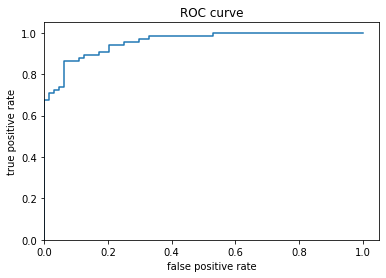
\includegraphics[width=0.4\textwidth]
        {images/BDT_ROC.png}}
        \caption{\label{fig:bdt_roc} The ROC curve for the BDT}
\end{figure}
\begin{figure}[!htb]
        \center{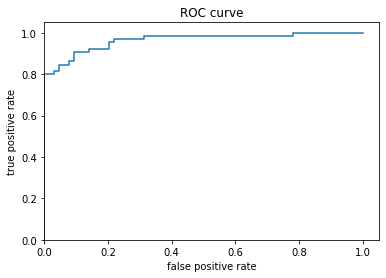
\includegraphics[width=0.4\textwidth]
        {images/NN_ROC.png}}
        \caption{\label{fig:bdt_roc} The ROC curve for the NN}
\end{figure}
Predictions produced by our models are of the form $[v_1,v_2]$, where $v_i$ is the probability that team $i$ won the series. Therefore, $[v_1,v_2]$ is a probability distribution, which was formed by normalizing the models' ``confidence" in team 1 winning the series and team 2 winning the series. Whichever is larger of the two is the predicted winner. Therefore, another interesting metric to examine is the distribution of the probability values for $v_1$. Here are the corresponding plots of these probability distributions:
\begin{figure}[H]
        \center{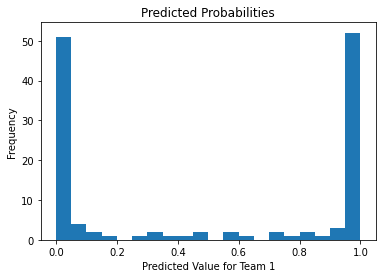
\includegraphics[width=0.35\textwidth]
        {images/BDT_prediction_probabilities.png}}
        \caption{\label{fig:bdt_prediction_distribution} The prediction probability distribution for the BDT}
\end{figure}
\begin{figure}[!htb]
        \center{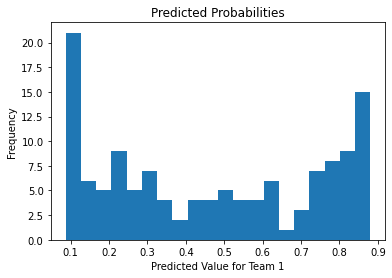
\includegraphics[width=0.35\textwidth]
        {images/NN_prediction_probabilities.png}}
        \caption{\label{fig:nn_prediction_distribution} The prediction probability distribution for the NN}
\end{figure}

Our models were trained using Google computing, with code hosted on Colab. 

\subsection{Discussion}
The boosted decision tree performed well on the data that was gathered. It was able to achieve 86\% accuracy and an AUC of 0.947. This was achieved using 300 steps, a learning rate of 0.1 and a max depth of 6. Through experimentation this hyperparameter configuration was found to produce the best BDT model in terms of accuracy. Increasing the max depth seemed to decrease the accuracy and AUC, although there were other configurations in which learning rate was decreased and number of steps was increased where the AUC was slightly better than the model above but the accuracy was approximately 3\% worse. The performance of this model is quite good, a 86\% percent accuracy means that we are achieving a relatively reliable prediction of the outcome of NBA series using the BDT. \\ \\
The neural network demonstrated very high performance on the dataset used, achieving a prediction accuracy of 89\% and an AUC of 0.964. The optimal layer/node configuration was discovered to be that of one hidden layer with 50 nodes. The number of nodes selected was not random: a commonly used heuristic is to have the number of nodes be between the input layer size and output layer size, which for our case was the range [2, 78]. Through experimentation, the optimal size of 50 was found. The sigmoid activation function was found to be most effective, as was the stochastic gradient descent learner algorithm with a learning rate of 0.001. Notable as well is the loss function; the sparse categorical cross-entropy loss function performed better than the binary cross-entropy one, despite the label class being binary. In general, the probabilistic loss functions, such as those above, significantly outperformed regression loss functions, such as mean squared error. Overall, the combination of all the optimal hyperparameters and configurations led to an excellent prediction accuracy of 89\%. \\ \\
With the dataset that was collected, the NN seems to outperform the BDT in every metric we recorded. From this we can say with some certainty that for the dataset we created, the NN is the superior model. The reasons for this are not particularly clear, but based on our knowledge of NNs we can assume that the ability of a NN to understand very complex relationships in data may have been one of the contributing factors. Our assumption prior to the testing was that the lack of data (only 644 total examples) would hinder the ability of a NN to accurately predict outcomes; this was incorrect. The BDT also performed well, which was expected due to the ability of BDTs to work well with relatively little data, but despite that advantage the BDT was outperformed by the NN. \\ \\
An interesting difference between the two models is the Predicted Probabilities distribution chart for both models. Each model produces predictions in the form [$v_1$, $v_2$], where $v_i$ is the model's confidence that team $i$ won the matchup, normalized so that they sum to 1. Thus, it is natural to examine each model's confidence in picking the winner/loser on average. Since $v_1$ and $v_2$ always sum to one, it is sufficient to plot just the $v_i$ values for $i = 1$. What we discovered was a large difference between the average confidence in the two models. The neural network had much less confidence in picking a winner on average, with over 70\% of the predictions being in the range (0.15, 0.85). In comparison, the BDT yielded extreme prediction values---in either (0.0, 0.1) or (0.9, 1.0)---over 90\% of the time. In essence, the BDT functioned as a binary switch whereas the NN was more akin to a true probability distribution, which we believe is evidence of better generalizing by the NN model. This hypothesis would help to explain the difference in accuracy between the two models. \\ \\
One of the somewhat shocking discoveries we made was how much better both our BDT and our NN models performed in comparison to our contemporaries. We achieved accuracy percentages in the high 80s, whereas none of our contemporaries seemed to be able to make predictions with percentage accuracy greater than mid-to-high 70s. This is most likely due to a key difference in the problem that other researchers addressed and the problem this paper addresses. Where they were all concerned with predicting the outcome of a single NBA basketball game in the regular season, this paper focused on predicting the outcome of a NBA playoff series. An NBA playoff series is a best of seven series, which means that up to 7 games are played and the first team to reach 4 victories wins the series. This best of seven format significantly reduces the likelihood that the inferior team stat-wise would win the matchup when compared to a singular game. In a single game, there is the possibility of a ``fluke"---an inferior team outperforming the superior team for any reason. As the name suggests, the chance of fluke occurring is low, and the probability is thus even lower for the event to occur 4 times over 7 games. We believe that this is why we were able to design models that significantly outperformed models from related work.

%%%%%%%%%. Conclusion and Future Work %%%%%%%%%

\section{Conclusion}

Over the last several years, the National Basketball Association has been continuously garnering a global audience, and every year their popularity increases. The world loves watching, playing, and talking about basketball. The annual revenues for the NBA increase likewise each year, from television broadcasting revenues, to ticket and merchandise purchases. Parallel to the growth of the NBA, we have seen an increase in the prevalence of sports betting, specifically focussed on the outcomes of NBA games. Therefore, the question of whether or not you can accurately predict the outcomes of these games is indivisibly linked to success in the betting pools. This paper discussed possible factors contributing to the outcomes of NBA playoff series, a natural way to organize the readily available game, season, and series data, as well as two industry-standard machine learning algorithms which may be used to predict playoff series outcomes. \\ \\
The first question this paper discussed was that of how much data could be collected and used, and in what format it should be stored. In order to draw correlations between two teams involved in a playoff matchup, it was decided that we would need to create a statistics aggregate, involving both teams' season average box scores, their average scores when pitted against each other in the regular season, and the outcome of their matchup in the playoffs. This way, we separated box scores from team names and players, to firstly avoid losing accuracy to sudden and major roster changes or injuries, but secondly to keep the scope of our project manageable. Obtaining and formatting the data was accomplished by the use of an open source Python API, as well as a custom HTML scraper application---also written in Python. After some simple list manipulations performed in Python, the data was saved to a CSV file. The custom application scraped and aggregated NBA team and series data from the 1997-98 season, up until the 2008-2019 season, accruing 644 examples. \\ \\ 
The main question this paper addresses is: ``what is the best machine learning algorithm and set of hyperparameters with which we may predict the outcomes of NBA playoff series". After some research into the topic, we decided to implement two industry-standard models: the Boosted Decision Tree (BDT) and the Neural Network (NN). Extending the concept of a decision tree, the BDT uses gradient boosting to train a series of smaller decision trees, and use them to minimize errors of future trees. The BDT model is known to perform well when faced with little data, and we knew from the onset of this project that the amount of data we could collect from the available NBA statistics was limited by the number of playoff series played in a season. On the other side of the coin, the NN excels at discovering and analyzing complicated relationships between different pieces of a real-valued training example. Since the number of statistics available for NBA games is many, we hypothesized that a NN would be strongly suited to analyzing our training examples---each of which contained 78 features. \\ \\
In terms of results, the standard metrics by which machine learning models are compared indicate that the NN marginally outperforms the BDT on our data set. The NN boasts a prediction accuracy and precision of around 90\%, with the BDT averaging around 86.5\% for each. Not only do our results exceed our expected statistics, but our models also significantly outperform the models presented by other researchers attempting a similar task. We believe the disparity between the results of our contemporaries and our own mainly stems from the possibility of an underdog team clutching a victory against the odds in the regular season being much higher than an underdog team defeating the favoured team in a best-of-7 playoff series. This difference would likely result in lower prediction accuracies for those models which attempt to predict arbitrary NBA games, whereas our models predict the outcome of playoff series. Despite having a higher prediction accuracy, we found that our NN implementation produced results with much less confidence on average than the BDT, which is why we see a large spread of the data for predicted probabilities in the NN, whereas for the BDT the data is simply bimodal. 

\section{Future Work}

We worked with a data set of some 600 training examples, because we were limited by the amount of data we could collect given our intentions of using it. If we were to continue this project, we would look to expand our data set into the other relevant basketball leagues, possibly to predict March Madness bracket outcomes for the NCAA. Moreover, we might look to apply our method to predicting the outcomes in other popular sporting events as well. In terms of improving our predictions in the NBA, the natural next step from here is to consider further which basketball metrics are indicators of victory/loss. In particular, we might incorporate performance indicators from specific players, especially the players who contribute most to a team's success. We wanted to keep the scope of the project manageable, so we did not want to attempt to formalize a player's contribution to a team, but in the world of basketball, many analysts, writers, and viewers hold the belief that the strength of a team is more reliant on their ``star" players---those who tend to perform the best under pressure---in the playoffs than they are in the regular season. So it would stand to reason that comparing the stats of the star players from opposing teams would give further insight into explaining who won. Another commonly held belief that we would be interested in testing is the notion of ``defense wins championships". The idea is that the defensive skill of a team matters most, and that a good defense will beat a good offense in high pressure situations like the NBA playoffs. Seeing as how the overwhelming majority of our features were offensive stats, this could be an opportunity to improve upon our accuracies. In the same vein, we might also begin to examine the effect injuries have on the outcomes of season games. \\ \\
Finally, it would be interesting to try incorporating past playoff success as a feature(s) in the dataset. A hypothetical example would be two features that give the best playoff result of both teams in the past 3 years, as well as two features for the number of playoff trips made in the past 5 years for each team. Sometimes we see the case where one team seems to have the upper hand for the entire game, only for the other team to make a few important plays as time is winding down and ``steal" the win. In this case, the typical basketball stats can not explain the result. It was most likely the significant playoff experience of the coach/some key players, or lack thereof in the losing team, that caused the turn of tide in the crucial moments. So, by modeling current and past intangible value in an NBA team's roster, as well as defensive abilities, we could vie for a prediction accuracy of greater than 90\%.

%%%%%%%%%. Bibliography %%%%%%%%%
\newpage
\bibliographystyle{aaai}
\bibliography{report}

\end{document}
